%
% This is a borrowed LaTeX template file for lecture notes for CS267,
% Applications of Parallel Computing, UCBerkeley EECS Department.
% Now being used for CMU's 10725 Fall 2012 Optimization course
% taught by Geoff Gordon and Ryan Tibshirani.  When preparing 
% LaTeX notes for this class, please use this template.
%
% To familiarize yourself with this template, the body contains
% some examples of its use.  Look them over.  Then you can
% run LaTeX on this file.  After you have LaTeXed this file then
% you can look over the result either by printing it out with
% dvips or using xdvi. "pdflatex template.tex" should also work.
%

\documentclass[twoside]{article}
\setlength{\oddsidemargin}{0.25 in}
\setlength{\evensidemargin}{-0.25 in}
\setlength{\topmargin}{-0.6 in}
\setlength{\textwidth}{6.5 in}
\setlength{\textheight}{8.5 in}
\setlength{\headsep}{0.75 in}
\setlength{\parindent}{0 in}
\setlength{\parskip}{0.1 in}

%
% ADD PACKAGES here:
%

\usepackage{amsmath,amsfonts,graphicx}

%
% The following commands set up the lecnum (lecture number)
% counter and make various numbering schemes work relative
% to the lecture number.
%
\newcounter{lecnum}
\renewcommand{\thepage}{\thelecnum-\arabic{page}}
\renewcommand{\thesection}{\thelecnum.\arabic{section}}
\renewcommand{\theequation}{\thelecnum.\arabic{equation}}
\renewcommand{\thefigure}{\thelecnum.\arabic{figure}}
\renewcommand{\thetable}{\thelecnum.\arabic{table}}

%
% The following macro is used to generate the header.
%
\newcommand{\lecture}[4]{
   \pagestyle{myheadings}
   \thispagestyle{plain}
   \newpage
   \setcounter{lecnum}{#1}
   \setcounter{page}{1}
   \noindent
   \begin{center}
   \framebox{
      \vbox{\vspace{2mm}
    \hbox to 6.28in { {\bf ROB501 - Fundamentals \& Emerging Topics in Robotics - Digital Control Systems } }
       \vspace{4mm}
       \hbox to 6.28in { {\Large \hfill Lecture #1 \hfill} }
       \vspace{2mm}
       \hbox to 6.28in { {\it Lecturer: #2 \hfill } }
      \vspace{2mm}}
   }
   \end{center}
   \markboth{Lecture #1}{Lecture #1}

   \vspace*{4mm}
}
%
% Convention for citations is authors' initials followed by the year.
% For example, to cite a paper by Leighton and Maggs you would type
% \cite{LM89}, and to cite a paper by Strassen you would type \cite{S69}.
% (To avoid bibliography problems, for now we redefine the \cite command.)
% Also commands that create a suitable format for the reference list.
\renewcommand{\cite}[1]{[#1]}
\def\beginrefs{\begin{list}%
        {[\arabic{equation}]}{\usecounter{equation}
         \setlength{\leftmargin}{2.0truecm}\setlength{\labelsep}{0.4truecm}%
         \setlength{\labelwidth}{1.6truecm}}}
\def\endrefs{\end{list}}
\def\bibentry#1{\item[\hbox{[#1]}]}

%Use this command for a figure; it puts a figure in wherever you want it.
%usage: \fig{NUMBER}{SPACE-IN-INCHES}{CAPTION}
\newcommand{\fig}[3]{
			\vspace{#2}
			\begin{center}
			Figure \thelecnum.#1:~#3
			\end{center}
	}
% Use these for theorems, lemmas, proofs, etc.
\newtheorem{theorem}{Theorem}[lecnum]
\newtheorem{lemma}[theorem]{Lemma}
\newtheorem{proposition}[theorem]{Proposition}
\newtheorem{claim}[theorem]{Claim}
\newtheorem{corollary}[theorem]{Corollary}
\newtheorem{definition}[theorem]{Definition}
\newenvironment{proof}{{\bf Proof:}}{\hfill\rule{2mm}{2mm}}

% **** IF YOU WANT TO DEFINE ADDITIONAL MACROS FOR YOURSELF, PUT THEM HERE:

\begin{document}

% Lecture Details
\lecture{3}{Asst. Prof. M. Mert Ankarali}


\section{Closed Loop Digital Control Systems}

Consider the fundamental DT-control system below 
%
    \begin{center}
\begin{minipage}[h]{\linewidth}
    \begin{center}
      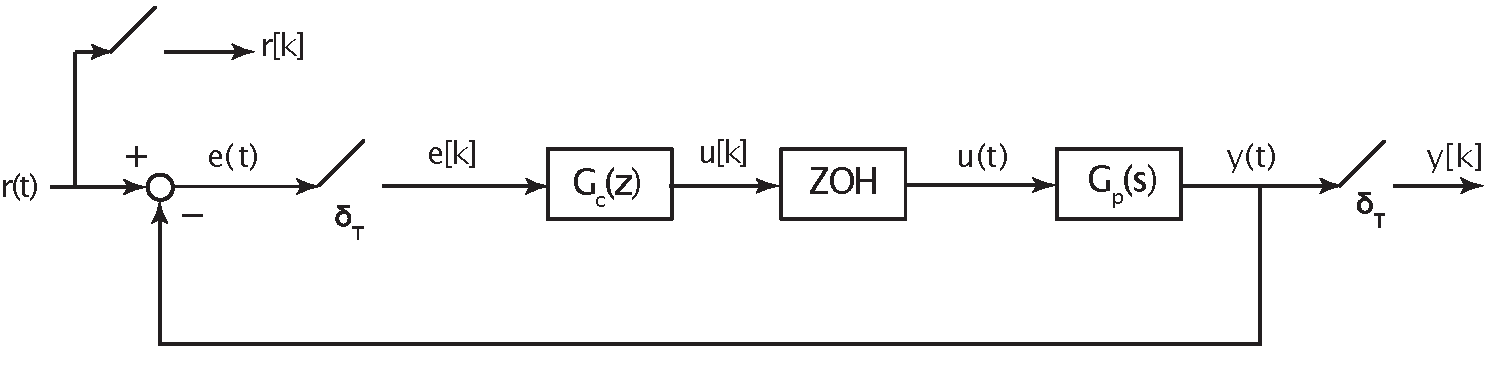
\includegraphics[width=\textwidth]{digitalblock}
    \end{center}
\end{minipage}
    \end{center}
%
Previously, we learned how to derive the transfer function of a fundamental open-loop digital control system composed of a ZOH operator, CT plant, and uniform sampler in cascaded form. We can use this derivation to find the transfer function from $u[k]$ to $y[k]$ such that 
%
\begin{align*}
\frac{Y(z)}{U(z)} = G_d(z) = \mathcal{Z}\left\lbrace 
\frac{G_p(s)}{s}  \right\rbrace
\end{align*}
%
Now let's derive the closed-loop transfer function from $r[k]$ to $y[k]$
%
\begin{align*}
E(z) &= R(z) - Y(z) \quad , \quad Y(z) = G_c(z) G_d(z) E(z) 
\\
E(z) &= R(z) - G_c(z) G_d(z) E(z)
\\
E(z) &= \frac{R(z)}{1 + G_c(z) G_d(z)}
\\
\frac{Y(z)}{R(z)} &= \frac{G_c(z) G_d(z)}{1 + G_c(z) G_d(z)}
\end{align*}
%
Note if we only care the signal flow in the sampled instants
we can re-draw the block diagram such that all time domain
signals are in DT and  all systems are represented in Z-domain.
The fundamental block diagram can be re-drawn as
%
    \begin{center}
\begin{minipage}[h]{0.75\linewidth}
    \begin{center}
      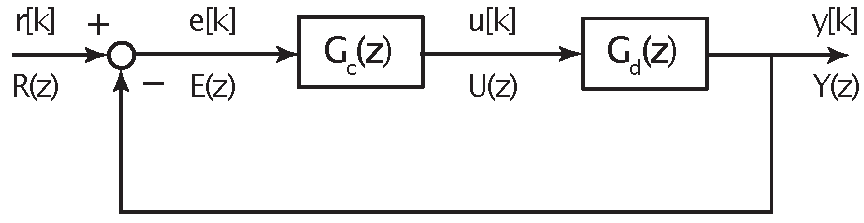
\includegraphics[width=\textwidth]{discreteblock}
    \end{center}
\end{minipage}
    \end{center}

\textbf{Example:} Let $G_p(s) = \frac{1}{s+1}$, $T=1$, $G_c(z) =
K$ (Discrete P Controller) . First find PTF (in z-domain).

\textbf{Solution:} First let's find $G_d(z)$ 
%
\begin{align*}
  G_d(z) &= (1 - z^{-1}) \mathcal{Z} \left\lbrace \frac{G_p(s)}{s}  \right\rbrace =
         \frac{1-e^{-1}}{z - e^{-1}} 
\end{align*}
%
which we already knew from the Lecture Notes 4. Now let's compute the
closed-loop PTF, $T(z)$.
%
\begin{align*}
T(z) =  \frac{G_c(z) G_d(z)}{1 + G_c(z) G_d(z)} = \frac{K(1 -e^{-1})}{z + K - (K+1) e^{-1}} 
\end{align*}
%
Let $\mathbf{K = 0.1}$, then compute the step-response of the closed-loop PTF
%
\begin{align*}
Y(z) &= R(z) T(z) = \frac{0.063 \, z}{(z-1)(z-0.3)}
\\
y[k] &= \mathcal{Z}^{-1} [ Y(z) ] = \left[  0.09 - 0.09 (0.3)^k
  \right] u[k]
\end{align*}
%
If we plot the step response we obtain the following plot
%
    \begin{center}
\begin{minipage}[h]{0.5\linewidth}
    \begin{center}
      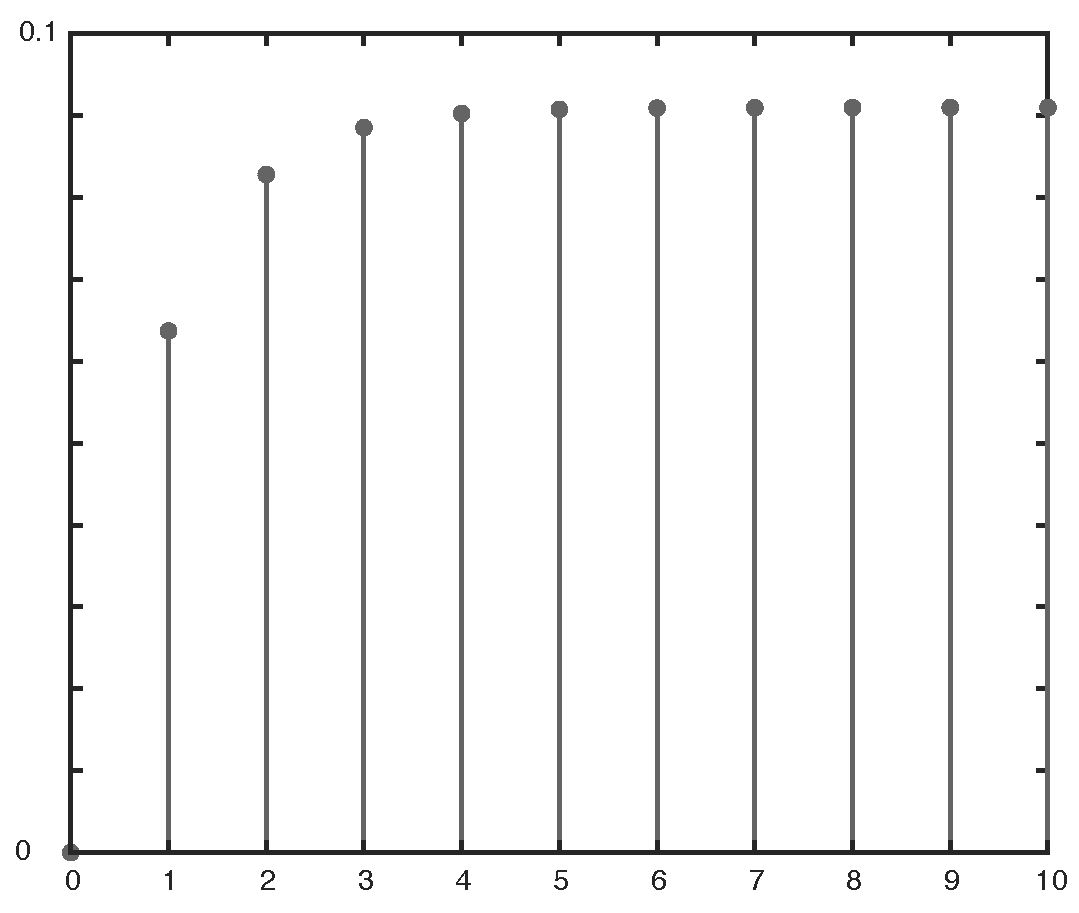
\includegraphics[width=\textwidth]{normal}
    \end{center}
\end{minipage}
    \end{center}
%

Now, Let $\mathbf{K = 1}$, then compute the step-response of the closed-loop PTF
%
\begin{align*}
Y(z) &= R(z) T(z) = \frac{z}{z-1} \frac{0.63}{z + 0.26} =
  \frac{0.63 \, z}{(z-1)(z+0.26)}
\\
y[k] &= \mathcal{Z}^{-1} [ Y(z) ] = \left[  0.5 - 0.5 (-0.26)^k
  \right] u[k]
\end{align*}
%
If we plot the step response we obtain the following plot
%
    \begin{center}
\begin{minipage}[h]{0.5\linewidth}
    \begin{center}
      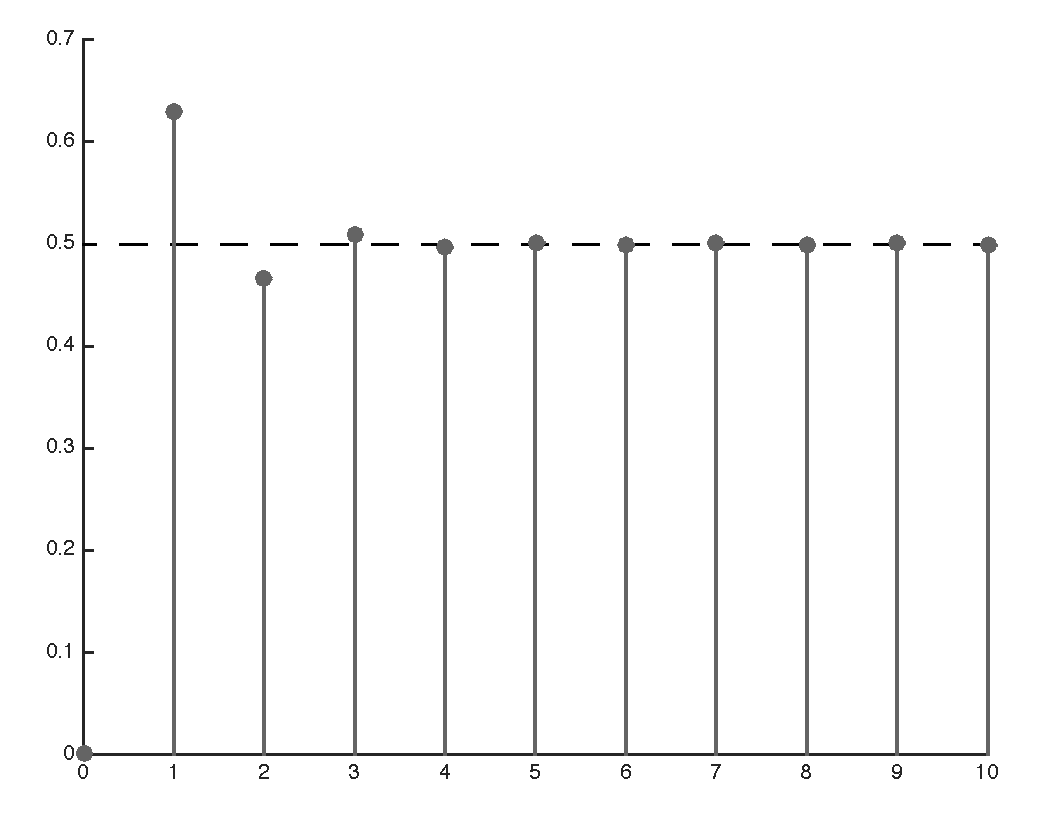
\includegraphics[width=\textwidth]{step}
    \end{center}
\end{minipage}
    \end{center}
%
What about inter-sample behavior? 

We can simulate the system and analyze the behavior. The figure below
shows the Simulink model as well as the output.
%
    \begin{center}
\begin{minipage}[h]{0.6\linewidth}
    \begin{center}
      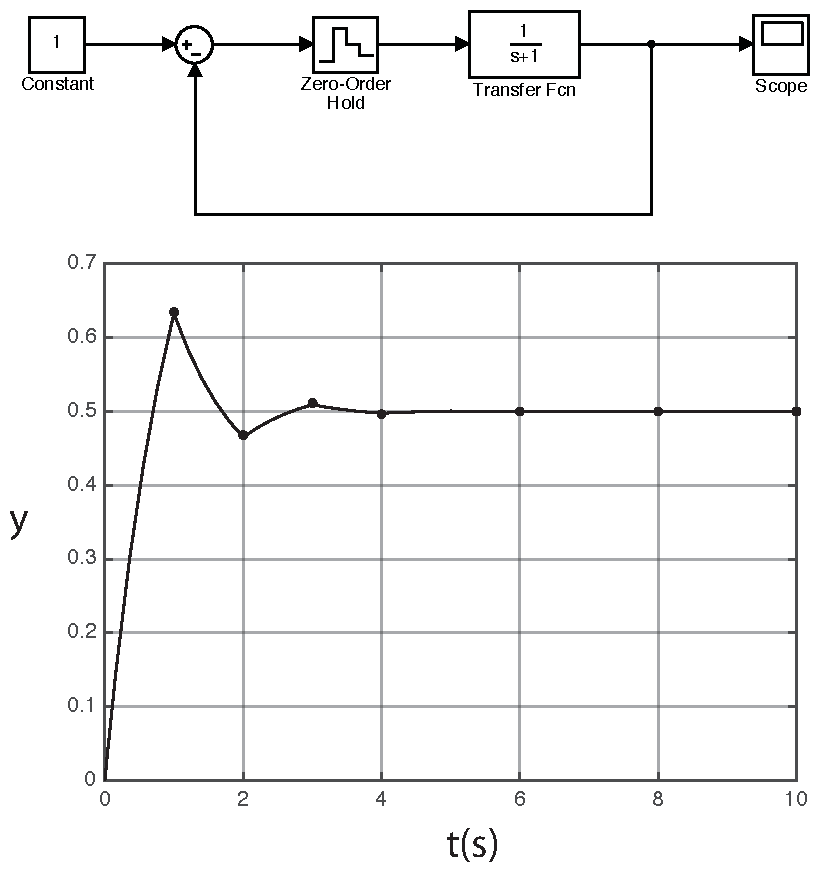
\includegraphics[width=\textwidth]{stepsimulink}
    \end{center}
\end{minipage}
    \end{center}
%
Now let $K = \frac{1+e^{-1}}{1-e^{-1}}$, then $Y(z)$ and $y[k]$
takes the form
%
\begin{align*}
Y(z) &= \frac{1.37 z}{(z-1)(z + 1)} 
\\
y[k] &= 0.69 - 0.69 (-1)^n
\end{align*}
%
The graph of $y[k]$ is illustrated below. It can be seen that the
output shows an oscillatory behavior.
%
    \begin{center}
\begin{minipage}[h]{0.5\linewidth}
    \begin{center}
      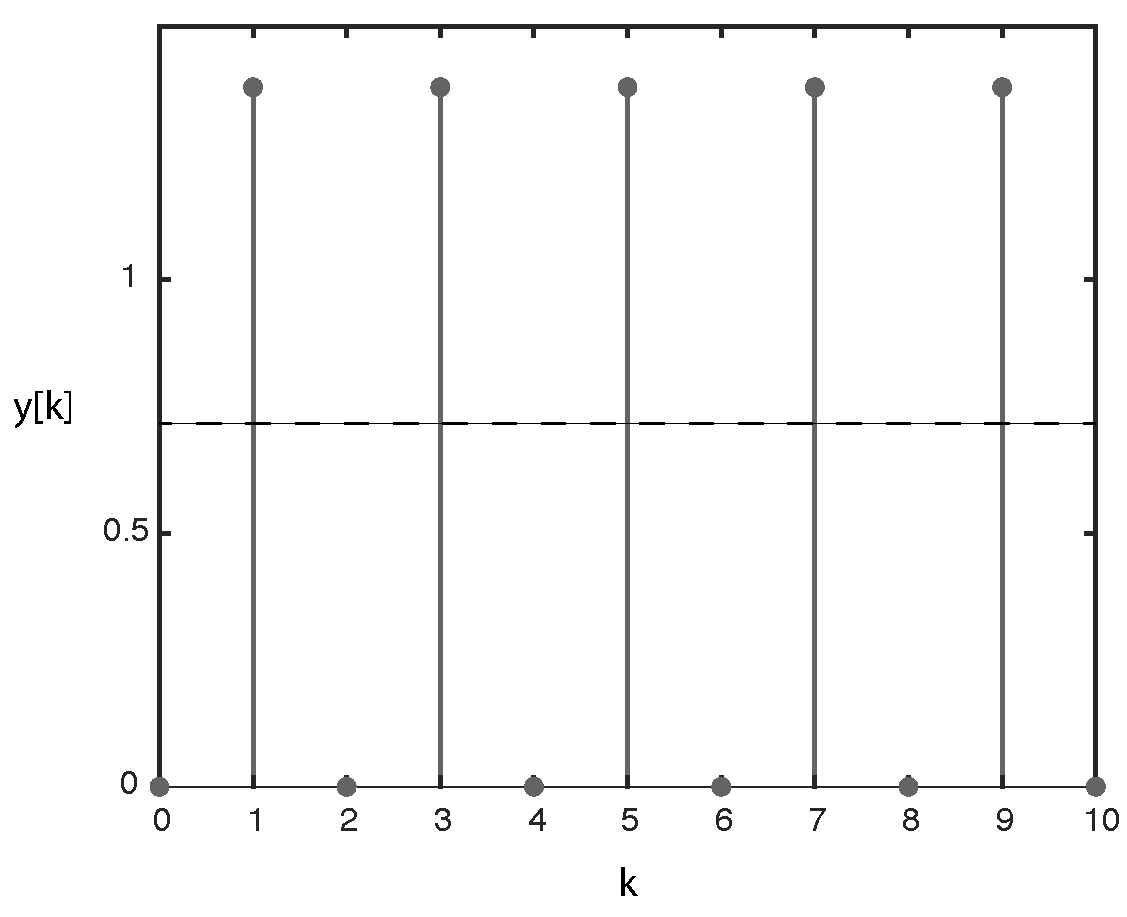
\includegraphics[width=\textwidth]{oscillate}
    \end{center}
\end{minipage}
    \end{center}
%
Now let $K = \frac{e^{-1}}{1-e^{-1}}$, then $Y(z)$ and $y[k]$
takes the form
%
\begin{align*}
Y(z) &= \frac{0.37}{z-1} 
\\
y[k] &= 0.37 u[k-1]
\end{align*}
%
Output converges to its steady state value in ``finite time''
(dead-beat behavior/controller). 

\textbf{Take home message:} It can be seen that even if the plant is
a simple first order transfer function, depending on the value of $K$,
we can observe very interesting behavior in the closed-loop DT system.

\newpage 

\section{Digital PID Controller}

In this section, we will try to obtain a form for the digital PID
controller. The continuous transfer function of a PID is given as
%
\begin{align*}
G_{PID}(s) = K_P + K_D s + \frac{K_I}{s}
\end{align*}
% 
One idea is to start from continuous PID form and then ``discretize''
it. One way of deriving a discrete controller, $G_{c}(z)$, is sampling 
the impulse response of the CT PID controller (or any controller) 
to obtain the impulse response of the DT PID controller.
Based in this approach if possible $G_c(z)$ simply commuted as
%
\begin{align*}
  G_c(z) = \mathcal{Z} \lbrace G_c(s) \rbrace
\end{align*}
%
Let's start with PI controller. 

\paragraph{Digitization of PI Controller:} It is a well known fact
that the PI Controller is in the form
%
\begin{align*}
   G_{PI}(s) = K_P + \frac{K_I}{s}
\end{align*}
%
The discretization simply gives
%
\begin{align*}
   G_{PI}(z) &= \mathcal{Z} \lbrace G_{PI}(s) \rbrace \\
&= K_P + K_I
  \frac{1}{1 - z^{-1}} \\
&= \frac{(K_I + K_P) - K_P z^{-1}}{1 - z^{-1}}
\\
&= \frac{b_0 + b_1 z^{-1}}{1 - z^{-1}}
\end{align*}
%
Now let's discretize PID controller which has the following CT
transfer function 
%
\begin{align*}
   G_{PID}(s) = K_P + K_D s + \frac{K_I}{s}
\end{align*}
%
The problem is $K_D  s$ term is non-causal. Let us approximate 
the effect of $K_D s$ in time domain and then perform a
discretization. A causal approximate derivative can be find 
by computing the backward difference.
%
\begin{align*}
 \frac{d x(t)}{dt} \approx \frac{x(t) - x(t-\Delta t)}{\Delta t}
\end{align*}
% 
Now let's compute the approximate derivative term at the sampling
instants and let $\Delta t = T$ we have 
%
\begin{align*}
 \frac{d x(t)}{dt}|_{t = kT} \approx \frac{x(k T) - x( (k-1) T)}{T}
\end{align*}
%
If we take the z-transform we can simply obtain a transfer function
for this FIR filter as
%
\begin{align*}
 G_{D}(z) = \frac{K_D}{T} (1 - z^{-1})
\end{align*}
%
Note that instead of $K_D / T$, we can just use $K_D$ for the gain. 
If we combine PI and D terms we obtain the following pulse transfer
function for the digital PID controller.
%
\begin{align*}
   G_{PID}(z) &= K_P + K_I
  \frac{1}{1 - z^{-1}}  + K_D \left(1 - z^{-1} \right)
\\
&= \frac{ K_P + K_D + K_I - (K_P + 2 K_D) z^{-1} + K_D z^{-2} }{ 1 -
  z^{-1} }
\\
&= \frac{b_0 + b_1 z^{-1} + b_2 z^{-2} }{ 1 -
  z^{-1} }
\end{align*}
%
The Figure below illustrates the frequency response characteristics of
an ideal CT-PID, a DT-PID, as well as an approximate causal CT-PID 
controllers. The transfer function of a causal CT-PID has the form
below
%
\begin{align*}
   G_{PID}(s) &\approx K_P + K_D \frac{s}{\gamma s + 1} +
                \frac{K_I}{s} \quad \mathrm{where ,}
                \\
     \gamma &> 0 \ \& \ \gamma \approx 0
\end{align*}
%
Qualitatively, at low and ``high'' frequencies all controllers behaves
similar. However, for some intermediate range of  frequencies there are significant
differences between the CT-PID and DT-PID (as well as approximate
causal CT-PID). Remarkably, for this frequency range DT-PID and approximate causal
CT-PID controllers' the frequency response polar polts are
qualitatively similar. This shows that if we choose the right
parameters, digitization of derivative term has a similar effect as
implementing an approximate analog derivative circuit. 
%
    \begin{center}
\begin{minipage}[h]{0.9\linewidth}
    \begin{center}
      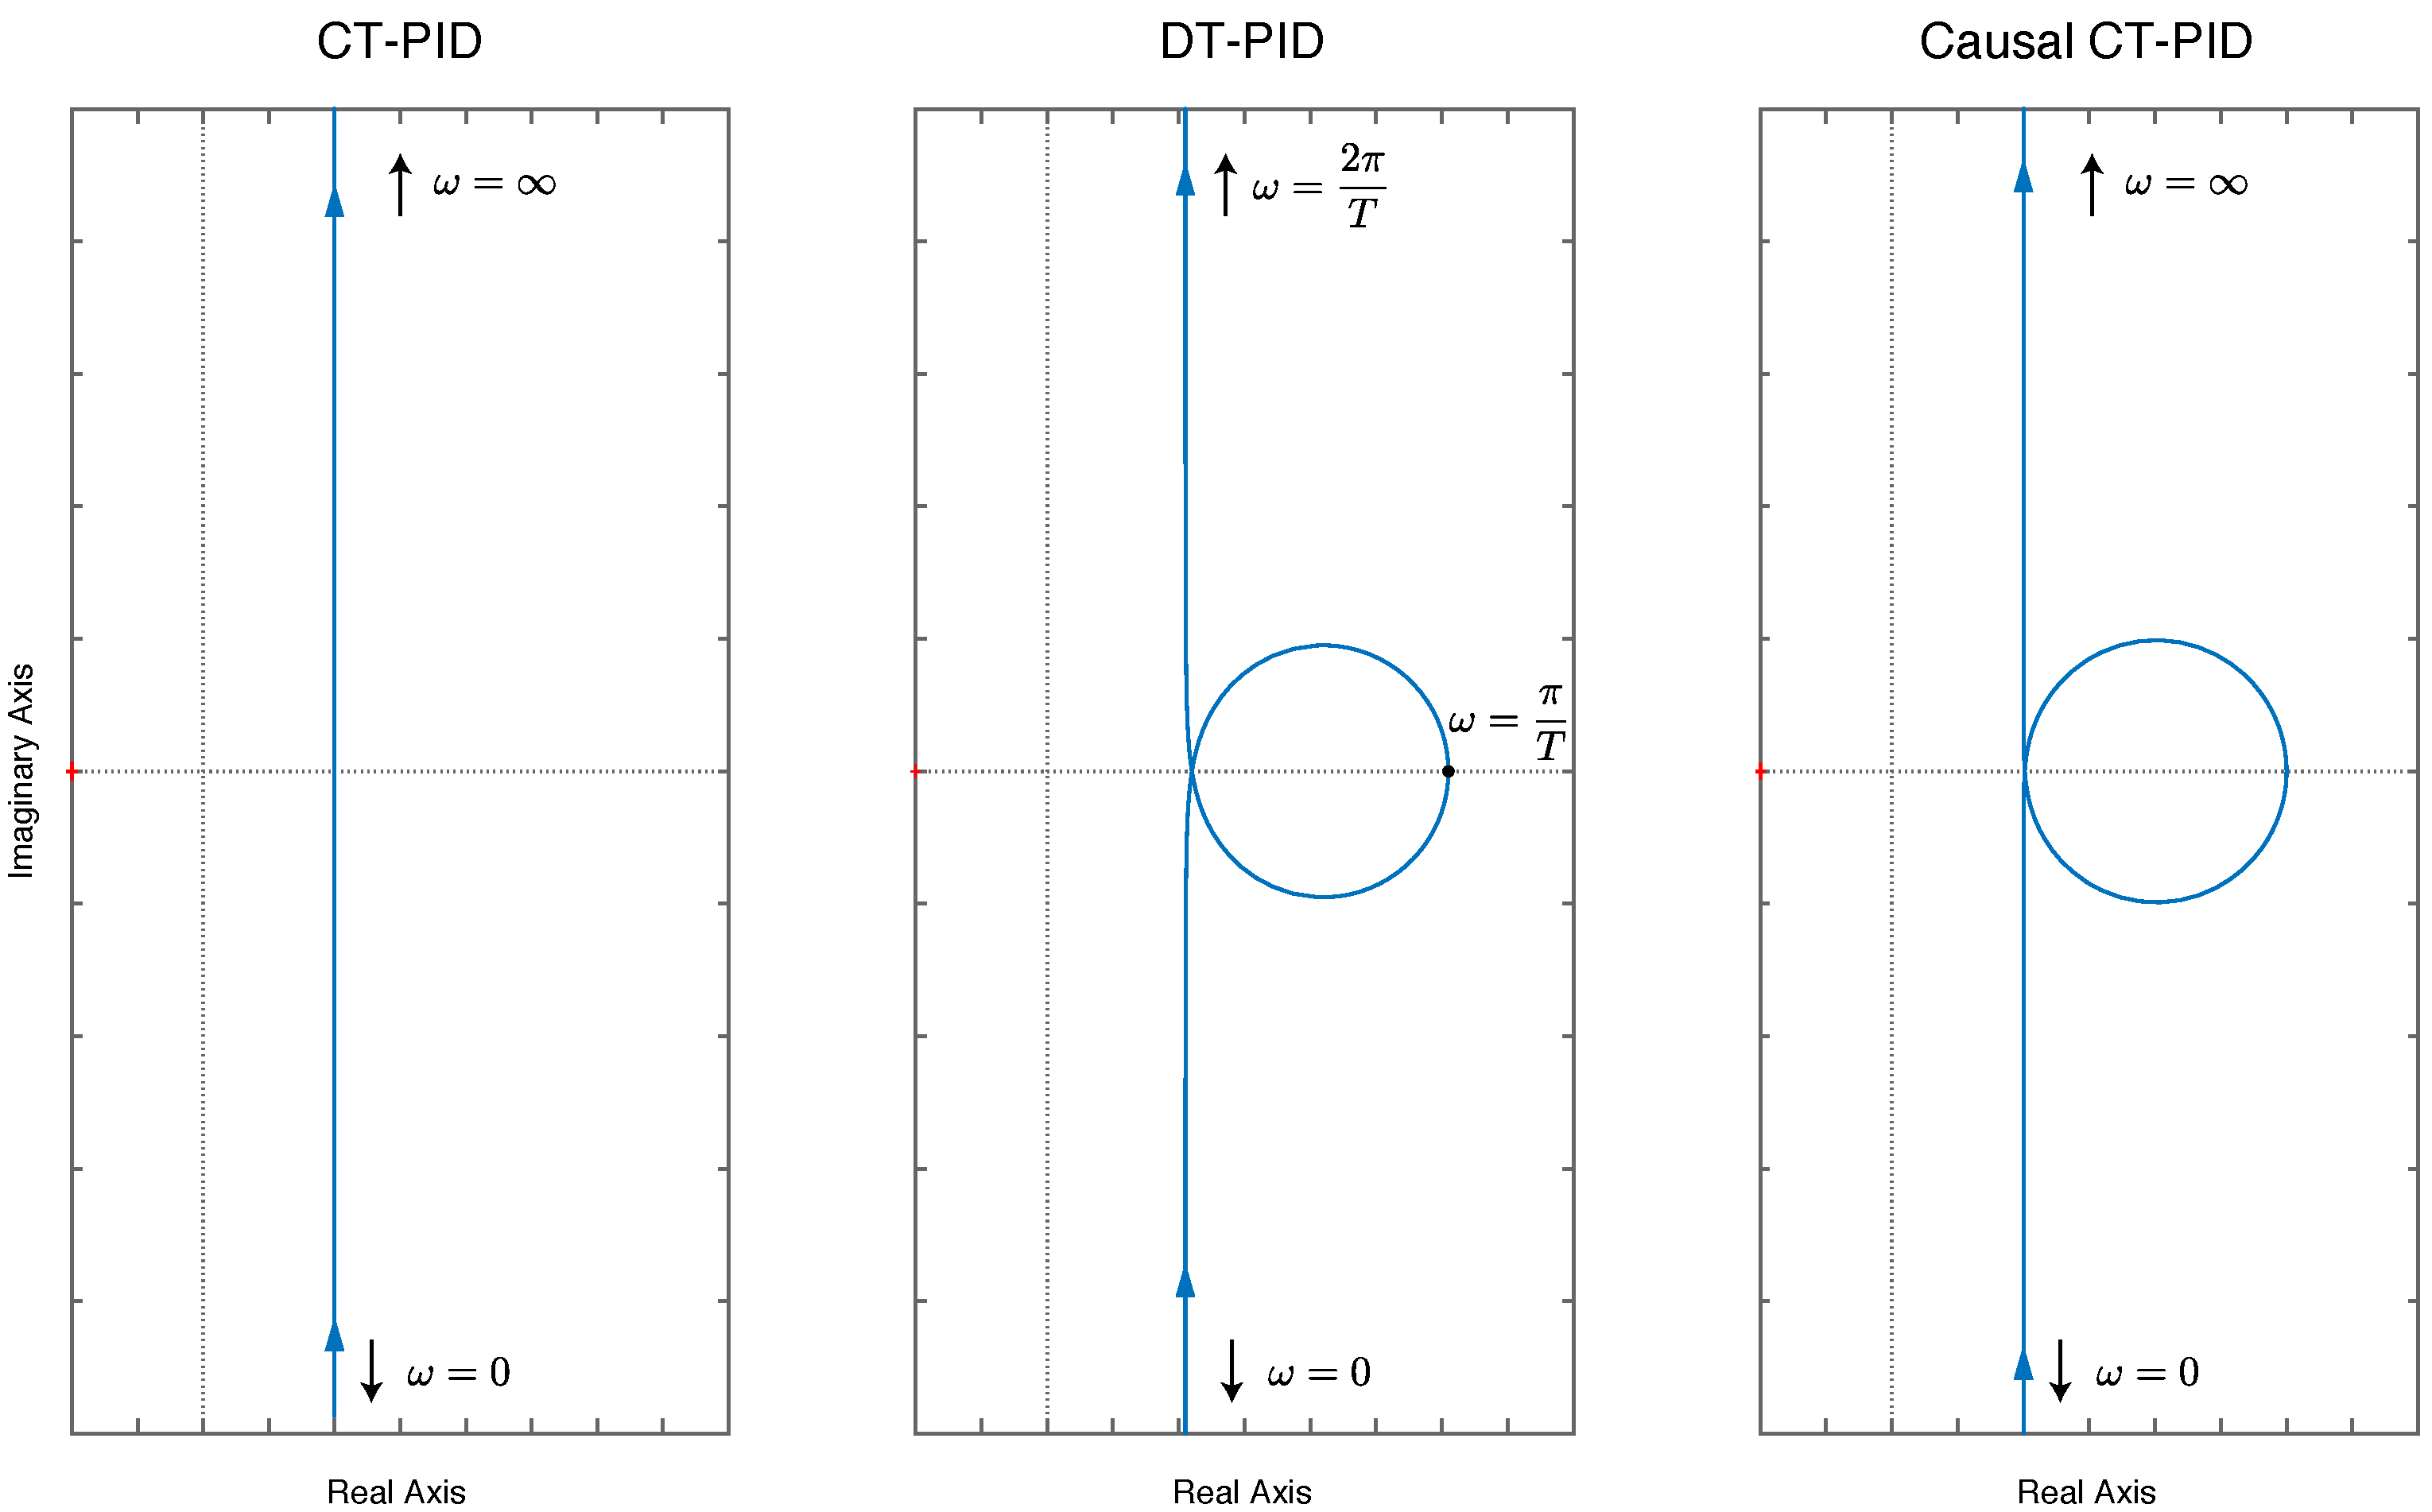
\includegraphics[width=\textwidth]{PID_Comp}
    \end{center}
\end{minipage}
    \end{center}
%

Note that frequency response function for CT and DT systems 
are found by the Fourier (CT or DT) transforms of the impulse
response functions, or simply they can be computed from
the s-domain or z-domain transfer functions
%
\begin{align*}
  \mathrm{CT:}& \quad G_c(s)|_{s = j\omega} = G_c(j \omega) \quad \\
  \mathrm{DT:}& \quad G_d(z)|_{z = e^{j\omega}} = G_d(e^{j\omega}) 
\end{align*}
%
Note that in DT case $\omega$ stands for DT frequency. Sometimes
$G_d(j\omega)$ or $G_d(\omega)$ used instead of $G_d(e^{j\omega})$.
We will cover the Frequency respons later in the class. 

\subsubsection*{PI \& PID Controllers with Leaky Integrator}
%
Some times for some practical and other considerations
instead of a true integrator (or accumulator) a leaky version 
is used. A leaky PI controller is in the form
%
\begin{align*}
  G_{L-PI}(s) &= K_P + K_I \frac{1}{s + \alpha} \\
  &= K_P \frac{s + ( \alpha + K_I / K_P) }{s + \alpha}
\end{align*}
%
where $\alpha > 0$ and $\alpha \approx 0$ (considering the bandwith 
of the closed loop system). It can be seen that a leaky-PI controller
has the same form with the compensator controller that we covered in 
302. If we obscure the frequency response characteristics of both
classical and leaky PI controllers, we observe that the behavior is
quite different at low frequencies but similar at high frequencies.
%
    \begin{center}
\begin{minipage}[h]{0.6\linewidth}
    \begin{center}
      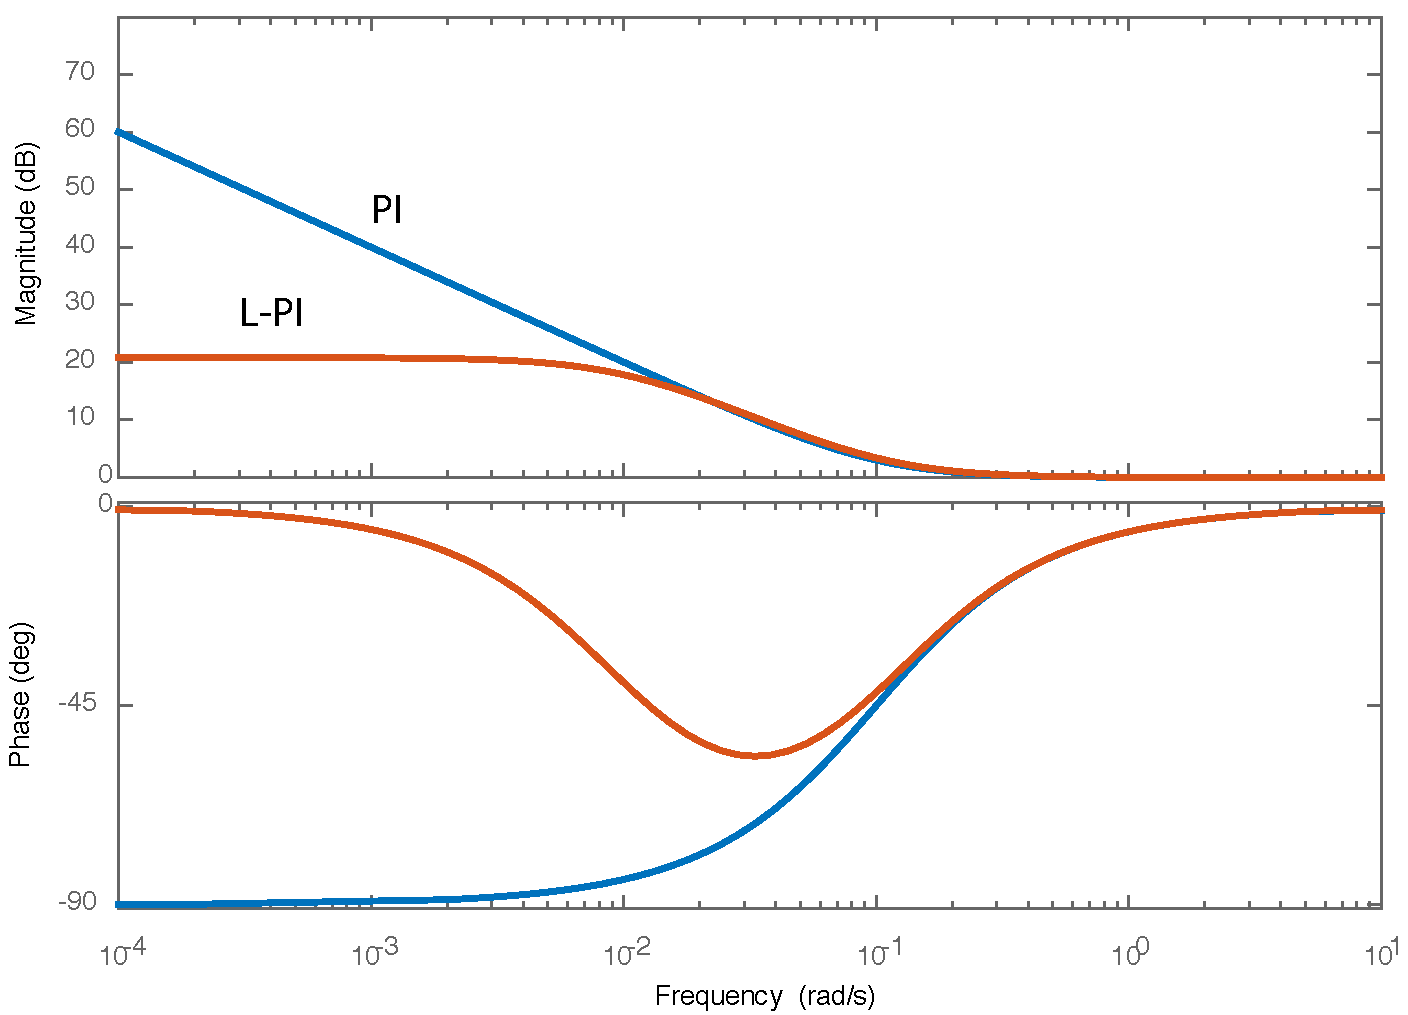
\includegraphics[width=\textwidth]{PI}
    \end{center}
\end{minipage}
    \end{center}
%
If we discretize this CT controller
using the emulation operation approach, we obtain
%
\begin{align*}
  G_{L-PI}(z) &= \mathcal{Z} \lbrace G_{L-PI}(s) \rbrace  = K_P + 
  \frac{K_I}{1 - e^{-\alpha T} z^{-1}} \\
  &= K_P  + \frac{K_I}{1 - \beta z^{-1}} 
  \\
  &= \frac{(K_P  + K_I) - K_P \beta z^{-1} }{1 - \beta z^{-1}} 
  \\
 &= \frac{ b_0 + b_1 z^{-1}}{1 + a_1 z^{-1}} 
\end{align*}
%
where similar to the CT case, $\beta < 1$ and $\beta \approx 1$.
Similar to the CT case, this DT transfer function has one zero and
one pole and it has the equivalent form with a DT-compensator 
controller. The bode plots of DT-PI and DT-Leaky-PI controllers
are illustrated in the Figure below. It can be seen that
at low frequencies the differences are significant,
but at high frequencies the responses between classical
and leaky PI controllers are very similar.
%
    \begin{center}
\begin{minipage}[h]{0.6\linewidth}
    \begin{center}
      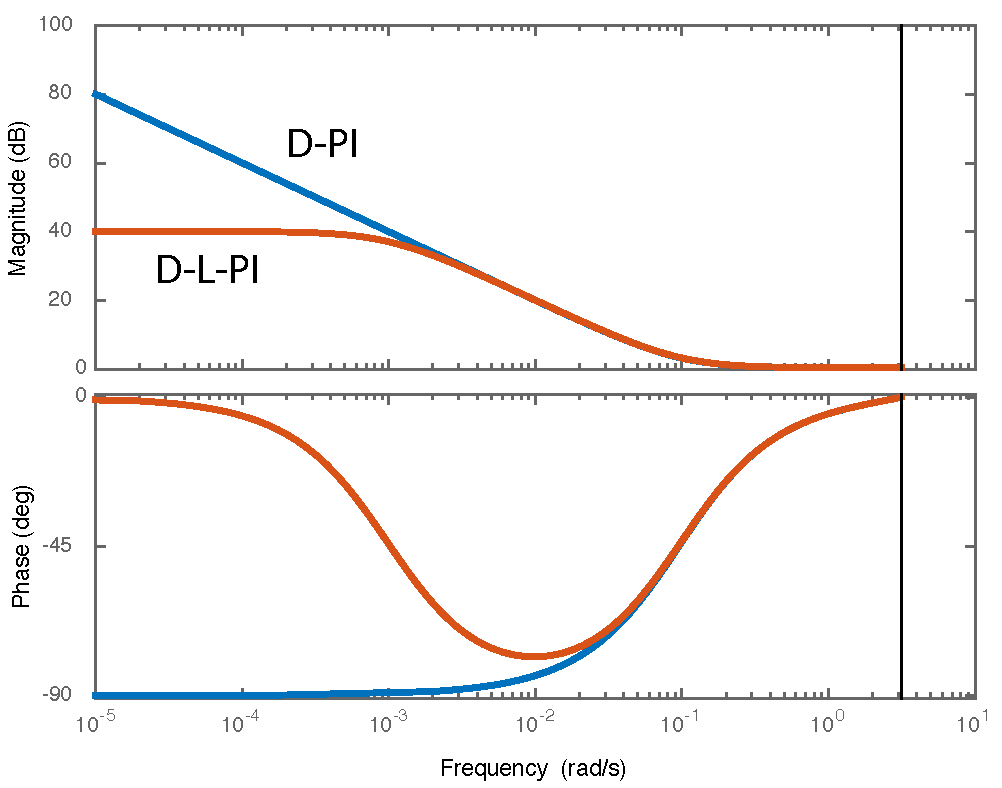
\includegraphics[width=\textwidth]{DPI}
    \end{center}
\end{minipage}
    \end{center}
%
One interesting result is that both for classical and leaky
cases, CT and DT frequency responses are qualitatively very 
similar. 

% **** This ENDS THE EXAMPLES. DON'T DELETE THE FOLLOWING LINE:
\end{document}
